\head{Февраль}{Листок 5. Теория множеств. Уровень 2.}

\begin{thm}
Докажите тождества\footnote{Т.е. равенства, верные для любых множеств $A$, $B$ и $X$.} \textit{(формулы де Моргана)}: 
\par
а)~$X \backslash (A \cup B) = (X \backslash A) \cup (X \backslash B)$;
\hfill
б)~$X \backslash (A \cup B) = (X \backslash A) \cup (X \backslash B)$.
\end{thm}

\begin{thm}
Ниже описаны два множества слов и словосочетаний. По какому принципу построены эти множества?

{\setlength{\intextsep}{2pt}
\begin{figure}[h]

\begin{minipage}{0.33\linewidth}
    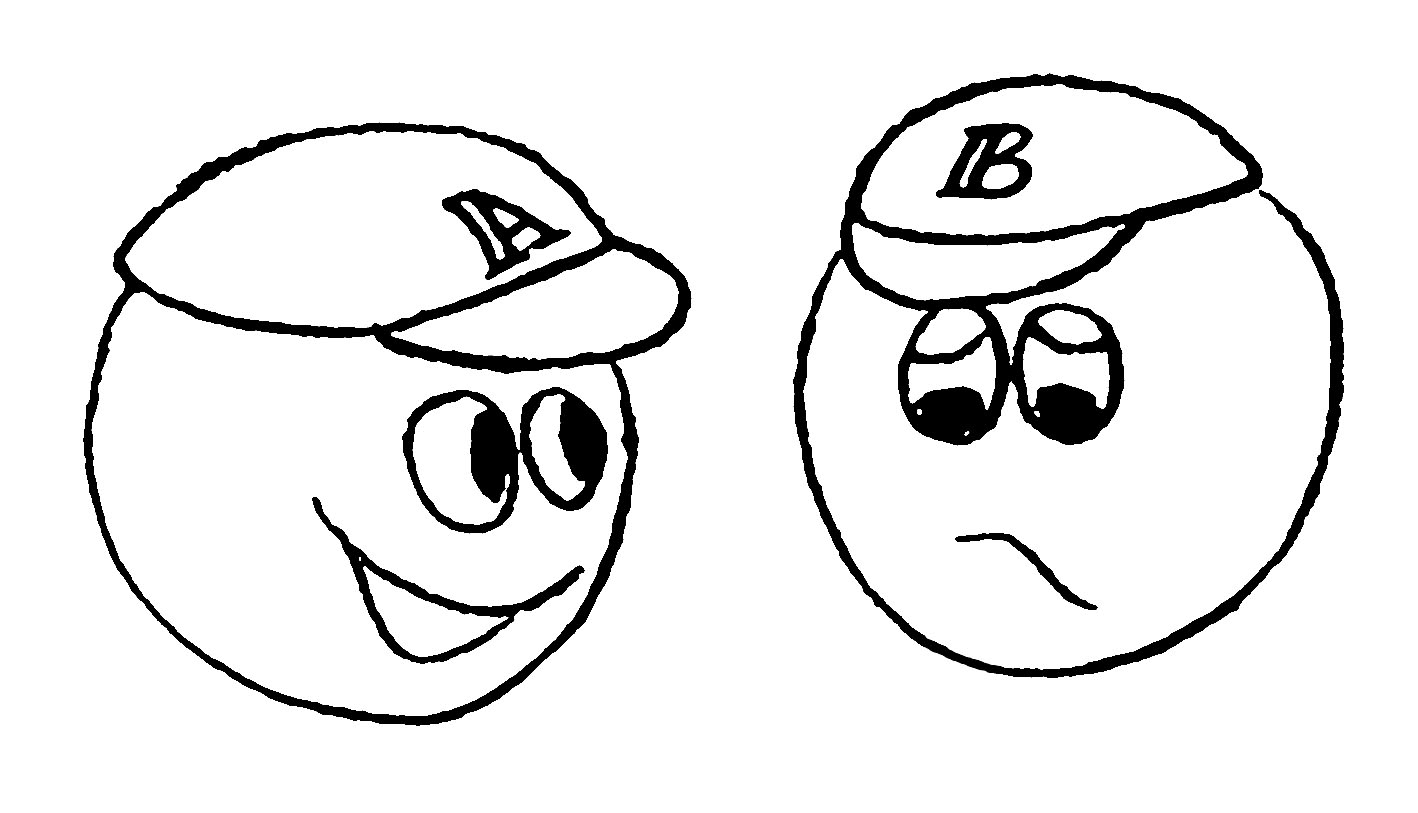
\includegraphics[scale=0.095]{img/veselo.png}
\end{minipage}
\hfill
\begin{minipage}{0.65\linewidth}\setlength{\parindent}{1.5em}
\centering
\begin{tabular}{cclll}
Множество A                                    & Множество B                                &  &  &  \\ \cline{1-2}
\multicolumn{1}{|c|}{русский}                  & \multicolumn{1}{c|}{английский}            &  &  &  \\ \cline{1-2}
\multicolumn{1}{|c|}{слово}                    & \multicolumn{1}{c|}{буква}                 &  &  &  \\ \cline{1-2}
\multicolumn{1}{|c|}{два слова}                & \multicolumn{1}{c|}{одно слово}            &  &  &  \\ \cline{1-2}
\multicolumn{1}{|c|}{сочетание слов}           & \multicolumn{1}{c|}{словосочетание}        &  &  &  \\ \cline{1-2}
\multicolumn{1}{|c|}{десять букв}              & \multicolumn{1}{c|}{девять букв}           &  &  &  \\ \cline{1-2}
\multicolumn{1}{|c|}{двадцатичетырехбуквенный} & \multicolumn{1}{c|}{двадцатитрехбуквенный} &  &  &  \\ \cline{1-2}
\end{tabular}
\end{minipage}

\end{figure}}

\end{thm}

\begin{thm}$^{\ast}$
Назовём слова (словосочетания) из множества $A$ в предыдущей задаче «весельчаковыми», а из множества $B$ – «грустняковыми». Придумайте слово (словосочетание), которое нельзя было бы отнести ни к «весельчаковому», ни к «грустняковому» множеству.
\end{thm}

\begin{thm}
Даны два множества (они могут пересекаться).
\par
а)~Сколько элементов в их объединении, если
известно, сколько в каждом из них и в их пересечении?
\par
б)~А если множеств 3?
\end{thm}

\begin{thm}
Решите задачу 20 для $n$ множеств.
\end{thm}

\begin{thm}
Поступили последние сведения о населении, являющемся гражданами Российской Федерации:
\par
1)~среди людей, которые едят абрикосы, есть и такие, которые не учатся в классах ТЛ <<ДваждыДва>>;
\par
2)~люди, играющие в пинг-понг, но не учащиеся классов ТЛ <<ДваждыДва>>, не едят морковку.
\par
Правда ли, что если русский не ест морковку – ещё не факт, что он не играет в пинг-понг?
\end{thm}